\tikzset{
  cuboid/.pic={
    \tikzset{%
      every edge quotes/.append style={midway, auto},
      /cuboid/.cd,
      #1
    }
    \coordinate (o) at (0, 0, 0);
    \coordinate (a) at (-\cubescale*\cubex,0,0);
    \coordinate (b) at (0,-\cubescale*\cubey,0);
    \coordinate (b1) at (0,0,-\cubescale*\cubez);
    \coordinate (c) at (b1) ++(\cubescale*\cubex,0,0);
    \coordinate (d) at (0,0,-\cubescale*\cubez);
    \coordinate (e) at (0,-\cubescale*\cubey,0);
    \coordinate (f) at (0,0,-\cubescale*\cubez);

    \draw [every edge/.append style={pic actions, densely dashed, opacity=.5}, pic actions]
    (o) -- ++(a) -- ++(b) edge coordinate [pos=1] (g) ++(b1) -- ++(\cubescale*\cubex,0,0) coordinate (c) -- cycle
    (o) -- ++(d) -- ++(e) edge (g) -- (c) -- cycle
    (o) -- ++(a) -- ++(f) edge (g) -- (d) -- cycle;
    ;
    \draw[fill=black!20, draw=black, thick] (o) circle (2pt);
    \draw[fill=black!20, draw=black, thick] (a) circle (2pt);
    \draw[fill=black!20, draw=black, thick] (b) circle (2pt);
    \draw[fill=black!20, draw=black, thick] (o) ++(a) ++(b) circle (2pt);
    \draw[fill=black!20, draw=black, thick] (g) ++(\cubescale*\cubex,0,0) circle (2pt);
    \draw[fill=black!20, draw=black, thick] (o) ++(d) circle (2pt);
    % \draw[fill=black!20, draw=black, thick] (o) ++(d) ++(e) circle (2pt);
    \draw[fill=black!20, draw=black, thick] (o) ++(a) ++(f) circle (2pt);
    \draw[fill=black!20, draw=black, thick] (g) circle (2pt);

  },
  /cuboid/.search also={/tikz},
  /cuboid/.cd,
  width/.store in=\cubex,
  height/.store in=\cubey,
  depth/.store in=\cubez,
  units/.store in=\cubeunits,
  scale/.store in=\cubescale,
  width=10,
  height=10,
  depth=10,
  units=cm,
  scale=.1,
}
\section{Volume Visualization}
$\bullet$ \textbf{Indirect} Volume Rendering (Marching Cubes, data is reduced to intermediate representation, which can then be rendered) \\
$\bullet$ \textbf{Direct} Volume Rendering (Ray Casting, data is considered semi-transparent with physical properties, and directly rendered) \\
$\bullet$ \textbf{Voxel}: point sample in 3D \\
$\bullet$ \textbf{Transfer Function}: maps data values to color \& opacity

\begin{center}
    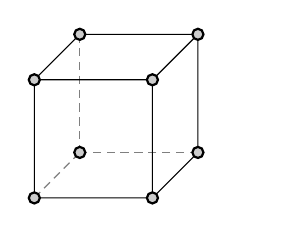
\begin{tikzpicture}
        \pic {cuboid={width=15, height=15, depth=15}};
    \end{tikzpicture}
\end{center}

\subsection{Transfer Function}
Associates distinct materials (value range) to distinct properties (color and opacity). Maps a different color to each scalar value.

$$T: \texttt{scalar value} \rightarrow color + \alpha$$

\subsection{Direct Volume Rendering}
Each \textbf{voxel} emits light of the color assigned to it, and absorbs light according to its opacity.

\subsection{Light Emission and Attenuation}
Volume rendering integral:
$$C(s) = \int_{s_0}^{s} C(s') \cdot e^{-\int_{s'}^s \alpha(t) \,dt} \,ds'$$

We are calculating the accumulated color until $C(s')$, with the absorption coefficient between the last color $s'$ and the point of view $s$.

\subsection{Ray Casting - Compositing}
\textbf{Front-to-back Strategy}

\begin{align*}
    C_{in} &= (0,0,0), \alpha_{in} = 0                         \\
    C_{out} &= C_{in} + (a - \alpha_{in}) \cdot \alpha \cdot C \\
    \alpha_{out} &= \alpha_{in} + (a - \alpha_{in}) \cdot \alpha    \\
\end{align*}

\newcommand{\eye}[4]% size, x, y, rotation
{   \draw[rotate around={#4:(#2,#3)}] (#2,#3) -- ++(-.5*55:#1) (#2,#3) -- ++(.5*55:#1);
    \draw (#2,#3) ++(#4+55:.75*#1) arc (#4+55:#4-55:.75*#1);
    % IRIS
    \draw[fill=gray] (#2,#3) ++(#4+55/3:.75*#1) arc (#4+180-55:#4+180+55:.28*#1);
    %PUPIL, a filled arc 
    \draw[fill=black] (#2,#3) ++(#4+55/3:.75*#1) arc (#4+55/3:#4-55/3:.75*#1);
}

\begin{center}
    \begin{tikzpicture}
        \coordinate (1) at (0, 1);
        \coordinate (2) at (0, 2.3);
        \coordinate (3) at (0, 2.8);
        \eye{0.5}{0}{0}{90};
        \draw[->] (1) -- (2);
        \node at (1, 0.7) {$C_{in}, \alpha_{in}$};
        \node at (3) {$C_{out}, \alpha_{out}$};

        \draw[pattern=north west lines, pattern color=blue] (-1, 1.8) rectangle (1, 1.5);
        \node at (1.5, 1.6) {$C, \alpha$};
    \end{tikzpicture}
\end{center}

\subsection{Direct Volume Rendering: Phong Shading}
We have to evaluate Phong's illumination model based on: \\
$\bullet$ \textbf{position} of current sample and light source \\
$\bullet$ sample's \textnormal{color} emission assigned by transfer function \\
$\bullet$ sample's \textbf{normal/gradient} (central difference)

\subsection{Gradient Estimation}
We can estimate the gradient using finite differencing. However, this technique is not feasible with large amounts of data.

\begin{align*}
    & \nabla f(x, y, z) \approx \\
    & \approx \frac{1}{2h} \begin{pmatrix}
        f(x + h, y, z) - f(x - h, y, z) \\
        f(x, y + h, z) - f(x, y - h, z) \\
        f(x, y, z + h) - f(x, y, z - h) \\
    \end{pmatrix}
\end{align*}

\subsection{Compositing Schemes}
$\bullet$ \textbf{Surface Rendering/First-Hit}: stop ray traversal if an ISOSurface is hit \\
$\bullet$ \textbf{Average}: simply accumulate colors, but ignore opacity \\
$\bullet$ \textbf{Maximum}: take maximum color along axis and display it